\documentclass[10pt,letterpaper]{article}
\usepackage[margin=0.5in]{geometry}
\usepackage{multicol}
\usepackage{amsmath,amssymb}
\usepackage{enumitem}
\usepackage{blindtext}
\usepackage{graphicx}

\setlength{\columnsep}{0.3in}
\pagestyle{empty}
\graphicspath{{images/}}

\begin{document}

\begin{multicols}{2}

\paragraph*{Sets}.\\
- $S = \{1,2,3,\dots\}$: Set Notation\\
- $x \in S$: x is an element of S.\\
- $x \notin S$: x is not an element of S.\\
- $\{1,2,3\}=\{3,2,2,1,2,3,1\}$: Order and repeated elements do not change equality.\\
- $\mathbb{R}$: set of all real numbers.\\
- $\mathbb{Z}$: set of all integers.\\
- $\mathbb{N}$: set of all natural numbers.\\
- $\mathbb{Q}$: set of all rational numbers.\\
- $\varnothing = \{\}$: the null set.\\
- $A = \{x \in S | P(x)\}$: A contains elements in S such that P(x) is true.\\
\textbf{Let} A and B be sets and $A,B \subseteq U$.\\
- $A \subseteq B$ if every element in A is in B.\\
- $A \subset B$ if every element in A is in B and at least one element in B is not in A.\\
- $A \times B = \{(a,b) | a \in A, b \in B\}$: Cartesian product of sets.\\
- $A = B \iff A \subseteq B \land B \subseteq A$\\
- $A \cup B = \{x : x \in A \lor x \in B\}$\\
- $A \cap B = \{x : x \in A \land x \in B\}$\\
- $B - A = \{x : x \in B \land x \notin A\}$\\
- $A^C = \{x : x \in U \land x \notin A\}$\\
- The \textbf{power set} of A ($\mathcal{P}(A)$), is the set of all subsets of A. 
--- If A has n elements, $\mathcal{P}(A)$ will have $2^n$ elements.

\paragraph*{Relations and Functions}.\\
- A relation R from A to B is a subset of $A \times B$: $R \subseteq A \times B$\\
- If $(x,y) \in R$, we say x is related to y by R.\\
- A is the domain of R and B is the codomain of R.\\
\textbf{Reflexive:} $\forall a \in A, (a,a) \in R$\\
\textbf{Symmetrics:} $\forall a,b \in A, (a,b) \in R \land (b,a) \in R$\\
\textbf{Antisymmetric:} $\forall a,b \in A, (a,b) \in R \land (b,a) \in R \implies a = b$\\
\textbf{Transitive:} $\forall a,b,c \in A, (a,b) \in R \land (b,c) \in R \implies (a,c) \in R$\\
\textbf{Equivalence Relations} are reflexive, symmetric, and transitive.\\
\textbf{Equivalence:} Is the set of outputs for a given input in a relation, for example for $5R2, 5R4, [5]=\{2,4\}$\\
\\
A function $F: A \rightarrow B$ is a relation with domain A and co-domain B such that:\\
- $\forall x \in A, \exists y \in B \ni (x,y) \in F$\\
- $\forall x \in A, \forall y,z \in B, (x,y) \in F \land (x,z) \in F \implies y=z$
\textbf{Onto:} $\forall x_1, x_2 \in X, f(x_1) = f(x_2) \implies x_1=x_2$\\
\textbf{One-to-One:} $\forall y \in Y, \exists x \in X \ni f(x) = y$\\

\paragraph*{Logical Form and Equivilence}.\\
An arguement is a sequence of statements aimed at demonstrating the truth of an assertion. The assertion at the end of the sequence is called the conclusion.
The statements that support the conclusion are called premises. If the premises are true, the conclusion must also be true.\\
\\
A logical statement is a declarative sentence that is either true or false, but not both.\\
- Not p: $\neg p$\\
- p and/but q: $p \land q$\\ 
- p or q: $p \lor q$\\
- Neither p nor q: $\neg p \land \neg q$\\
\\
Two logical statements are equivilent ($\equiv$) if they have the same truth tables.\\
De Morgan's Laws:\\
- $\neg(p \land q) \equiv \neg p \lor \neg q$\\
- $\neg(p \lor q) \equiv \neg p \land \neg q$

\paragraph*{Conditional Statements}.\\
The statement ``If p then q'' is denoted as $p \implies q$, and read ``p implies q''.\\
Order of operations: $(), \neg, \land/\lor, \implies$\\
- $p \implies q \equiv \neg p \lor q$\\
- $\neg (p \implies q) \equiv p \land \neg q$\\
- Contrapositive of $p \implies q$ is $\neg q \implies \neg p$\\
- Converse of $p \implies q$ is $q \implies p$\\
- Inverse of $p \implies q$ is $\neg p \implies \neg q$

\paragraph*{Valid and Invalid Arguments} Let $p_n$ represent each premise of an argument and c represent the conclustion of an arguement.\\
- An argument form is valid when $(p_1 \land p_2 \land \dots \land p_n) \implies c$
\begin{center}
    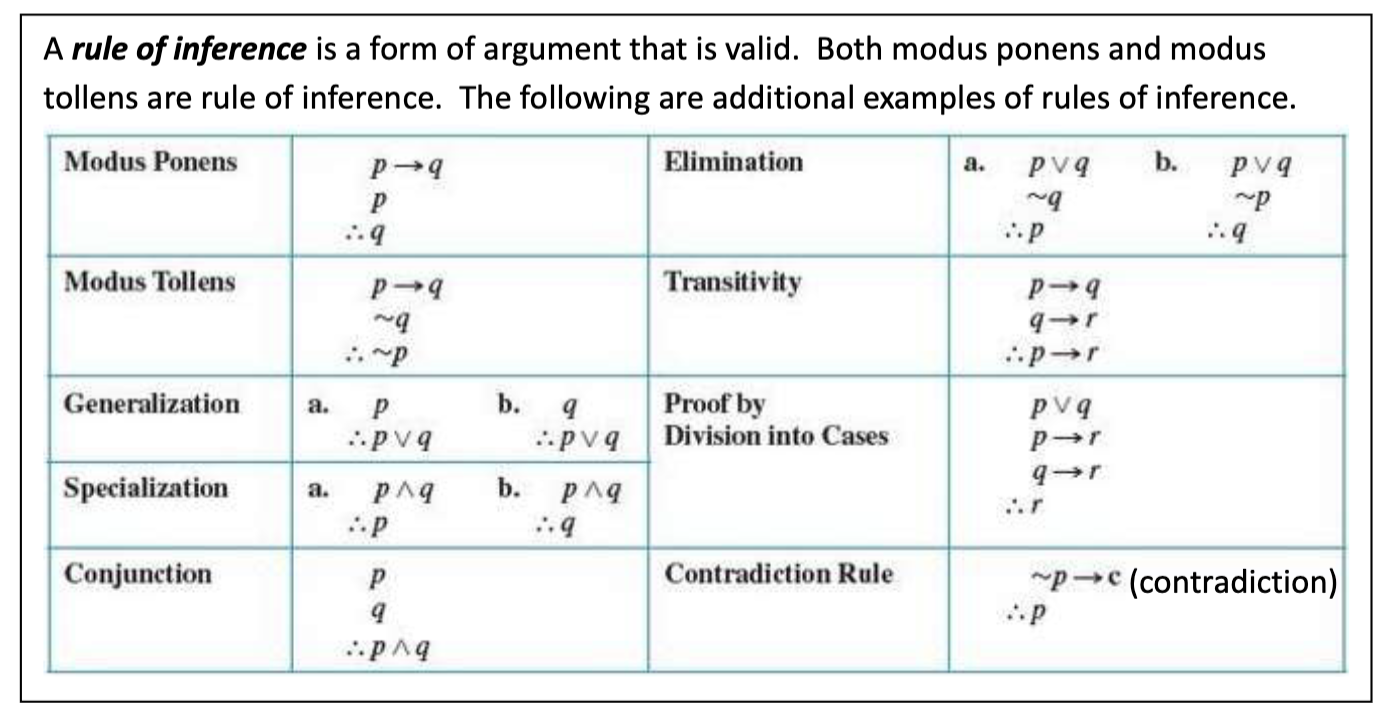
\includegraphics[width=0.45\textwidth]{rule-of-inference.png}
\end{center}

\paragraph*{Predicates and Quantified Statements} A predicate is a sentence that contains a finite number of variables and becomes a statement when specific values are substituted for the variables. 
The Domain of a predicate is the set of all values that can be substituted for the variable. If P(x) is a predicate with domain D, the truth set of P(x) is the set of all elements in D 
for which P(x) is true when they are substituted for x. The truth set of P(x) is denoted by $\{x \in D \ni P(x)\}$\\
- Universal Statement -- $\forall x \in D, P(x)$\\
- $\neg(\forall x \in D, P(x)) \equiv \exists x \in D \ni \neg P(x)$\\
- Existential Statement -- $\exists x \in D \ni P(x)$''\\
- $\neg(\exists x \in D \ni P(x)) \equiv \forall x \in D, \neg P(x)$\\
\textbf{Consider the satement:} $\forall x \in D, P(x) \implies Q(x)$\\
- Negation: $\exists x \in D \ni P(x) \land \neg Q(x)$\\
- Contrapositive: $\forall x \in D, \neg Q(x) \implies \neg P(x)$\\
- Converse: $\forall x \in D, Q(x) \implies P(x)$\\
- Inverse: $\forall x \in D, \neg P(x) \implies \neg Q(x)$

\paragraph*{Divisibility} If n and d are integers and d $\neq$ 0, then n is divisible by d if and only if n = dk for some integer k. This is notated $d|n$ (d divides n).\\
- $d|n \iff \exists k \in \mathbb{Z} \ni n=dk$\\


\end{multicols}

\newpage

\begin{multicols}{2}

\begin{center}
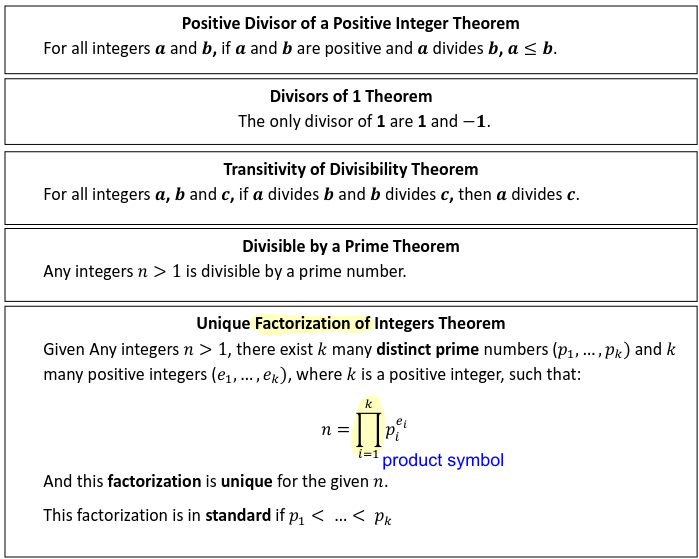
\includegraphics[width=0.4\textwidth]{divisibility-theorems.png}
\end{center}

\paragraph*{Number Theory}.\\\\
\textbf{Odd and Even Numbers (Parity Property):}\\
- Even: $\forall n \in \mathbb{Z}, 2|n \iff \exists k \in \mathbb{Z} \ni n = 2k$\\
- Odd: $\forall n \in \mathbb{Z}, \neg{2|n} \iff \exists k \in \mathbb{Z} \ni n = 2k + 1$\\
\textbf{Rational Numbers}\\
- $\forall n \in \mathbb{Q}, \exists a,b \in \mathbb{Z} \ni n = \frac{a}{b} \land b \neq 0$\\
\textbf{The Triangle Inequality}\\
- $\forall x,y \in \mathbb{R}, |x+y| \leq |x| + |y|$\\
\textbf{Quotient Remainder Theorem}\\
- $\forall n \in \mathbb{Z}, \forall d \in \mathbb{Z}^+, \exists q, r \in \mathbb{Z} \ni n = dq + r \land 0 \leq r < d$\\
- In simpler terms: $n \div d = q, \quad n \mod d = r$\\
\textbf{Zero Product Property}\\
If neither of two real numbers is zero, then their product is non-
zero. The contrapositive of this theorem is also true: If the product of two
real numbers is zero, then at least one of the two numbers is zero.\\
- Let $a,b \in \mathbb{Q}$\\
- $ab = 0 \implies a = 0 \lor b = 0$\\
- $ab \neq 0 \implies a \neq 0 \land b \neq 0$\\


\paragraph{Methods of Proof}.\\\\
\textbf{Constructive Proof of $\exists x\in D \ni Q(x)$:}\\
- Find an x in D such that Q(x) is true.\\
- Give Directions for finding such an x in D\\
\textbf{Disproving $\forall x \in D, P(x) \implies Q(x)$ by counterexample:}\\
- Find an x in D that makes P(x) true, but Q(x) false.\\
\textbf{Method of Exhaustion of Proving $\forall x \in D, P(x) \implies Q(x)$:}\\
- Check all x in D to make sure that when P(x) is true, Q(x) is false.\\
\textbf{Direct Proof of $\forall x \in D, P(x) \implies Q(x)$:}\\
- Suppose x is an arbitrary element in D for which the hypothesis P(x) is true.\\
- Using definitions or previously established results and rules to conclude Q(x) is true.\\
\textbf{Proof by Division into cases:}\\
- Each case gets it's own argument form. For example, running a proof in the case n is even and odd.\\
\textbf{Proof by Contradiction}\\
- Suppose the opposite of the to-be proved conclusion.\\
- Show that this supposition leads logically to a contradiction (a statement that is always false).\\
- Conclude that the statement to be proved is true.\\
\textbf{Proof by Contraposition}\\
- Express the given statement in the form of ``$\forall x \in D, P(x) \implies Q(x)$''\\
- Rewrite as contrapositive: ``$\forall x \in D, \neg Q(x) \implies \neg P(x)$''\\
- Prove the contrapositive by direct proof:\\
--- Suppose $\exists x \in D \ni \neg Q(x)$\\
--- Prove $\neg P(x)$\\
\textbf{Proof by Induction} of $\forall n \in \{a \in \mathbb{Z} : n \geq a\}, P(n)$\\
- Basis step: Show that $P(a)$ is true where a is the lower bound of the range.\\
- Inductive Step: Suppose $P(k)$ is true, then prove $P(k+1)$\\
\textbf{Proof by Strong Induction} involves proving all base cases if multiple are given.

\textbf{Sequences}\\
- $\sum_{i=m}^{n} a_i + \sum_{i=m}^{n} b_i = \sum_{i=m}^{n}(a_i + b_i)$\\
- $c \cdot \sum_{i=m}^{n} a_i = \sum_{i=m}^{n}(c \cdot a_i)$\\
- $\prod_{i=m}^{n} a_i \cdot \prod_{i=m}^{n} b_i = \prod_{i=m}^{n}(a_ib_i)$\\
- $\sum_{i=0}^{n} r^i = \frac{r^{n+1} - 1}{r - 1}$\\
- Arithmetic Sequence: $a_k = a_{k-1} - d = a_0 + nd$\\
- Geometric Sequence: $a_k = r \cdot a_{k-1} = a_0 \cdot r^n$\\
\textbf{Binomial Coefficient} (choose r items from n choices)\\
- $nCr = \binom{n}{r} = \frac{n!}{r!(n-r)!}$\\

\vspace{9999pt}

\end{multicols}

\end{document}